\chapter{Quelques méthodes dérivées}\label{Ch-XFEM}
\begin{abstract} Dans ce court chapitre, nous survolons quelques méthodes également utilisées en simulation numérique. Nous n'entrons pas dans le détail, mais si les notions d'éléments finis, de formulations mixtes et hybrides et les multiplicateurs de Lagrange ont été comprises, alors nos courtes explications doivent suffire.
\end{abstract} %
%%%%----------------------------------------------------------
%\section{Les volumes finis}

%\medskip
%\section{Les volumes finis}

\medskip
\section{Méthode des éléments frontières}\label{Sec-BEM}\index{élément fini!frontière}
%%%%----------------------------------------------------------
La méthode des éléments finis et la \textcolorblue{méthode des éléments frontière}\index{élément fini!frontière} peuvent être considérées comme issues des méthodes de Ritz\index[aut]{Ritz (Walther), 1878-1909, Suisse} et de Trefftz\index[aut]{Trefftz (Erich Immanuel), 1888-1937, Allemand} respectivement. Dans les deux cas, il s'agit de résoudre un problème décrit par des équations aux dérivées partielles dans un domaine~$\Omega$ et sur sa frontière~$\Gamma=\partial\Omega$ en remplaçant le problème continu par un nombre fini de paramètres inconnus dans la résolution numérique.

\medskip
La méthode de Ritz\index[aut]{Ritz (Walther), 1878-1909, Suisse}, et donc la méthode des éléments finis, se base sur l'existence d'un principe variationnel pour lequel la fonction inconnue sera recherchée comme une combinaison de fonctions de base définies dans tout le domaine~$\Omega$.

\medskip
La méthode de Trefftz\index[aut]{Trefftz (Erich Immanuel), 1888-1937, Allemand} a été proposée en 1926 dans un article intitulé <<~une alternative à la méthode de Ritz~>>. Le passage domaine/frontière se fait en appliquant Green\index[aut]{Green (George), 1793-1841, Anglais} à la formulation variationnelle considérée et en proposant des fonctions d'interpolation linéairement indépendantes qui satisfont les équations aux dérivées partielles d'intérieur de domaine \emph{a priori}. Trefftz montre que l'intégrale d'intérieur de domaine du principe variationnel disparaît et que seules subsistent des intégrations aux frontières. \textcolorred{Cependant, cette méthode discrétisant la frontière seule peut être employée uniquement
si le problème physique considéré est gouverné par des équations différentielles linéaires et homogènes.}
On obtient encore un système de type~$\MM{K}\VV{q}=\VV{F}$, mais les intégrales se font uniquement
sur~$\Gamma$.

\medskip
La méthode des éléments finis et la méthode des éléments frontières\index{élément fini!frontière} sont toutes deux des méthodes très robustes pour de nombreuses applications industrielles, ce qui en fait des outils de choix pour les simulations numériques. Cependant, leur utilisation pose des problèmes lorsque l'on a évolution des surfaces internes à cause du <<~maillage~>> de ces surfaces: description correcte, évolution de ces surfaces, fissures, front de sollicitation, interfaces... Une des motivations pour les méthodes sans maillage est de s'affranchir de ces difficultés.



\medskip
\section{Méthodes sans maillage}\label{Sec-meshless}\index{méthode sans maillage}

Depuis le début des années 90, de nombreuses méthodes sont apparues où la discrétisation ne repose plus sur un maillage mais sur un ensemble de points\footnote{On peut par exemple nommer la méthode des éléments diffus, la méthode de Galerkin sans éléments (Element Free Galerkin Method, EFGM), Reproducing Kernel Particle Method (RKPM), $h-p$ Cloud Method...}. \textcolorred{Chaque point possède un domaine d'influence de forme simple}, comme un cercle, sur lequel les fonctions d'approximation sont construites. Les différentes approches se distinguent, entre autres, par les techniques utilisées pour la construction des fonctions d'approximation. Ces fonctions sont construites de manière à pouvoir représenter tous les modes rigides et de déformation sur le domaine d'influence (c'est une condition nécessaire à la convergence de ces méthodes), et sont nulles en dehors. On écrira alors:
\begin{equation}
u(x) = \dsum_{i\in N_s(x)}\dsum_{\alpha=1}^{N_f(i)} a_i^\alpha \phi_i^\alpha(x)
\end{equation}
où~$N_s(x)$ est l'ensemble des points~$i$ dont le support contient le point~$x$ et~$N_f (i)$ est le nombre de fonctions d'interpolation définies sur le support associé au point~$i$.

\medskip
Une fois les fonctions d'interpolation construites, il est possible d'en ajouter d'autres par \textcolorblue{enrichissement}. L'enrichissement de l'approximation permet ainsi de représenter un mode de déplacement donné~$F(x)\phi_i^\alpha(x)$:
\begin{equation}
u(x) = \dsum_{i\in N_s(x)}\dsum_{\alpha=1}^{N_f(i)} a_i^\alpha \phi_i^\alpha(x) + \dsum_{i\in N_s(x)\cap N_f}\dsum_{\alpha=1}^{N_f(i)} b_i^\alpha\phi_i^\alpha(x)F(x)
\end{equation}
L'enrichissement des fonctions d'interpolation a par exemple permis de résoudre des problèmes de propagation de fissure en deux et trois dimension sans remaillage: la fissure se propage à travers un nuage de points et est modélisée par enrichissement, à savoir des fonctions~$F(x)$ discontinues sur la fissure ou représentant la singularité en fond de fissure.

\medskip
Les \textcolorblue{méthodes sans maillage (Meshless Methods)}\index{méthode sans maillage} sont flexibles dans le choix de l'approximation et de l'enrichissement. En revanche, le choix du nombre de points d'intégration et de la taille du domaine d'influence dans un nuage arbitraire de points d'approximation n'est pas trivial: alors que dans le cas de la méthode des éléments finis, la matrice de rigidité est obtenue par assemblage des contributions élémentaires, pour les méthodes sans maillage, l'assemblage se fait en couvrant le domaine de points d'intégration et en ajoutant leur contribution. Qui plus est, les conditions aux limites de type Dirichlet sont délicates à imposer.



\medskip
\section{Partition de l'unité}\label{Sec-partition}\index{partition de l'unité}
\textcolorred{La base des éléments finis classiques peut elle-aussi être enrichie} (afin de ne pas recourir aux méthodes sans maillage) de manière à représenter une fonction donnée sur un domaine donné.
Melenk\index[aut]{Melenk (Jens Markus), ?- , Autrichien} et
Babu\u{s}ka,\index[aut]{Babuška (Ivo Milan), 1926-, Tchèque}
en 1996, ont appelé cette technique:
la \textcolorblue{Partition de l'Unité (PU)}.
Ils ont remarqué en fait que si~$N_s(x)$, autrement dit l'ensemble des points~$i$ dont le support contient le point~$x$, était remplacé par~$N_n(x)$, c'est-à-dire l'ensemble des nœuds contenant~$x$, alors on retombait sur la formulation éléments finis usuelle, qui, sous forme <<~assemblée~>> s'écrivait bien alors:
\begin{equation}
u(x) = \dsum_{i\in N_n(x)}\dsum_{\alpha} a_i^\alpha \phi_i^\alpha(x)
\end{equation}
\textcolorgreen{Cela veut simplement dire que, dans le cas des éléments finis, on considère les supports
comme liés à des nœuds, alors que dans le cas sans maillage, ils sont liés à des points. En d'autres
termes, si l'on considère un nœud à chaque point, la méthode des éléments finis est un cas particulier de la méthode
sans maillage.} On peut alors également écrire l'approximation de partition de l'unité par:
\begin{equation}
u(x) = \dsum_{i\in N_n(x)}\dsum_{\alpha} a_i^\alpha \phi_i^\alpha(x) + \dsum_{i\in N_n(x)\cap N_f}\dsum_{\alpha} b_i^\alpha\phi_i^\alpha(x)F(x)
\end{equation}



\medskip
\section{Méthode des éléments finis étendue}\label{Sec-XFEM}\index{méthode des éléments finis étendue}\index{X-FEM}
Dans le cas particulier où la méthode de partition de l'unité\index{partition de l'unité} est appliquée à la modélisation de discontinuités ou de vides au sein même des éléments, on obtient alors la \textcolorblue{méthode des éléments finis étendue (X-FEM)}:\index{méthode des éléments finis étendue}\index{X-FEM}
\begin{equation}
\begin{aligned}
u(x) &= \dsum_{i\in I}u_i\phi_i(x) + \dsum_{i\in L} a_i\phi_i(x) H(x)\\
&\qquad\qquad + \dsum_{i\in K_1}\phi_i(x)\biggl(\dsum_{j=1}^4b_{i,1}^jF_1^j(x)\biggr) + \dsum_{i\in K_2}\phi_i(x)\biggl(\dsum_{j=1}^4b_{i,2}^jF_2^j(x)\biggr)
\end{aligned}
\end{equation}
où~$I$ est l'ensemble des nœuds du maillage, $L$ l'ensemble des nœuds enrichis pour modéliser la fissure coupant de part en part un élément, $K_1$ et~$K_2$ les nœuds enrichis pour modéliser le fond de fissure.

\medskip
L'avantage en X-FEM\index{méthode des éléments finis étendue}\index{X-FEM} est qu'il n'est plus demandé au maillage de se conformer à des surfaces, qu'elles soient intérieures ou extérieures, et qu'il peut alors être conservé lors de leur évolution. Les surfaces ne sont plus maillées et sont localisées sur le maillage grâce à la notion de \textcolorred{fonction de niveau}. À chaque nœud au voisinage de cette surface, on associe la distance signée à cette surface. Cette fonction <<~distance~>> peut être interpolée sur chaque élément avec les fonctions classique de premier ordre. Les surfaces sont ainsi stockées par un champ élément fini défini au voisinage de la surface qui participe au calcul au même titre que les autres champs physiques. En particulier, la X-FEM\index{méthode des éléments finis étendue}\index{X-FEM} permet la modélisation des trous, sans avoir à forcer le maillage à se conformer à ceux-ci. Un nœud dont le support est complètement à l'intérieur du trou ne donne pas lieu à la création de ddl. Pour un nœud dont le support coupe la frontière du trou, la fonction d'interpolation classique est multipliée par une fonction valant 1 dans la matière et 0 dans le trou.

\medskip
\section{Méthodes particulaires}\label{Sec-PBM}\index{méthode particulaire}
La dénomination <<~méthodes particulaires~>> recouvre deux types différents de modèles pour la mécanique du solide et pour la mécanique des fluides. D'un côté, on trouve des concepts de discrétisation dans lequel la réponse d'un continuum est projetée sur les <<~particules~>> véhiculant l'information mécanique au cours de leurs déformations: ce sont typiquement les \textcolorblue{méthodes sans maillage, Smoothed Particles Hydrodynamics (SPH), Moving Particle Simulation (MPS), Particle Finite Element Method (PFEM), Material Point Method (MPM) et Lattice-Boltzmann-Method (LBM).}\index{méthode de Lattice-Boltzmann}\index[aut]{Boltzmann (Ludwig), 1944-1906, Autrichien} Lissé Hydrodynamique Particules (SPH), Simulation particule en mouvement (MPS), méthode des éléments finis de particules (PFEM), Méthode point matériel (MPM) et le Réseau-Boltzmann-Méthode (LBM). De l'autre côté, cette notion exprime la représentation de calcul de particules physiques existantes à différentes échelles: ce sont typiquement les méthodes \textcolorblue{Molecular Dynamics (MD) et Discrete (Distinct) Element Method (DEM).} ou la méthode des éléments discrets (Distinct) (DEM). On peut alors considérer les cas où les particules existent physiquement (comme pour les matières granulaires) ainsi que les cas où elles évoluent au cours du processus de chargement; ces deux cas pouvant même éventuellement être couplés.

\medskip
Comme nous ne pouvons tout présenter, nous proposons de survoler la méthode de Lattice-Boltzmann,\index[aut]{Boltzmann (Ludwig), 1944-1906, Autrichien} notamment parce qu'elle est utilisée en acoustique.

\medskip
\subsection{Méthodes de treillis de Boltzmann}\index{méthode de Lattice-Boltzmann}\index[aut]{Boltzmann (Ludwig), 1944-1906, Autrichien}
Dans les \textcolorblue{méthodes de treillis de Boltzmann} (lattice Boltzmann Methods = LBM), on ne cherche plus à simuler un problème de dynamique des fluides par les équations de Navier-Stokes\index[aut]{Navier (Claude Louis Marie Henri), 1785-1836, Français}\index[aut]{Stokes (George Gabriel), 1819-1903, Anglais}\index{équations!de Navier-Stokes} (nous avons déjà évoqué certains problèmes que l'on rencontre alors), mais en se servant de l'équation de Bolzmann\index[aut]{Boltzmann (Ludwig), 1944-1906, Autrichien} discrète pour un fluide newtonien avec modèle de collision (par exemple Bhatnagar-Gross-Krook).\index[aut]{Bhatnagar (Prabhu Lal), 1912-1976, Indien}\index[aut]{Krook (Max), 1913-1985, Américain}\index[aut]{Gross (Eugène P.), 1926-1991, Américain} L'idée est de simuler l'écoulement ainsi que les processus de collision entre un nombre limité de particules. Les interactions entre particules conduisent à un comportement de l'écoulement visqueux applicables à une échelle plus grande. On peut donc les voir également comme des méthodes de décomposition de domaine ou d'homogénéisation [paragraphe~\ref{Sec-dec} et chapitre~\ref{Ch-Homog}].

\medskip
Les LBM sont particulièrement bien adaptées à la simulation de fluides autour de géométries complexes et ont l'avantage de pouvoir être implémentées sur des machines parallèles. Bien qu'historiquement développées pour les gaz en treillis, elles s'obtiennent également directement à partir des équations simplifiées de Boltzmann BGK (Bhatnagar-Gross-Krook).\index[aut]{Bhatnagar (Prabhu Lal), 1912-1976, Indien}\index[aut]{Krook (Max), 1913-1985, Américain}\index[aut]{Gross (Eugène P.), 1926-1991, Américain}

On considère un treillis discret dont les nœuds portent des particules. Ces particules sautent d'un nœud au suivant selon leur vitesse: c'est la phase de propagation. Puis les particules se choquent et acquièrent une nouvelle vitesse: c'est la phase de collision. La simulation procède en alternant les phases de propagations et de collisions des particules. On montre que de tels gaz suivent les équations des fluides de Navier-Stokes.\index{équations!de Navier-Stokes}\index[aut]{Navier (Claude Louis Marie Henri), 1785-1836, Français}\index[aut]{Stokes (George Gabriel), 1819-1903, Anglais} L'inconvénient majeur de cette méthode appliquée à la dynamique des fluides est l'apparition de <<~bruit~>>. Si l'on ne cherche qu'un champ relativement calme (peu de variations, en tous cas, pas de variations brutales), il est nécessaire de pouvoir prendre la moyenne sur un treillis relativement grand et sur une grande période de temps. Dans ce cas, les LBM contournent le problème en pré-moyennant le gaz: on considère la distribution des particules sur le treillis plutôt que les particules elles-mêmes.

\medskip
La forme générale de l'équation de treillis de Boltzmann est:
\begin{equation}
f_i(x+\Delta_t \vect{c_i}, t+\Delta_t) = f_i(x,t) + \Omega_i
\end{equation}
où~$f_i$ est la concentration de particules se déplaçant avec la vitesse~$\vect{c_i}$ jusqu'au nœud suivant pendant un temps~$\Delta_t$.~$\Omega_i$ représente l'opérateur de collision, et c'est lui qui change d'une méthode à l'autre. Dans le modèle BGK (Bhatnagar-Gross-Krook).\index[aut]{Bhatnagar (Prabhu Lal), 1912-1976, Indien}\index[aut]{Krook (Max), 1913-1985, Américain}\index[aut]{Gross (Eugène P.), 1926-1991, Américain}, la distribution des particules après propagation est relaxée vers la distribution à l'équilibre~$f_i^{eq}$, et on a:
\begin{equation}
\Omega_i = \frac1{\tau}\left(f_i(x,t)-f_i^{eq}(x,t)\right)
\end{equation}
avec~$\tau$ le paramètre de relaxation, qui détermine la viscosité cinématique~$\nu$ du fluide selon la relation~$\nu=(2\tau -1)/6$. La distribution à l'équilibre est une fonction de la densité locale~$\rho$ et de la vitesse locale~$\vect{u}$, qui sont les moments d'ordre 1 et 2 de la distribution des particules:
\begin{equation}
\rho(x,t) = \dsum_i f_i(x,t) \qquad\text{ et }\qquad \vect{u}(x,t)=\dfrac{\sum_i f_i(x,t)\vect{c_i}}{\rho(x,t)}
\end{equation}
Cette distribution à l'équilibre est calculée par la relation:
\begin{equation}
f_i^{eq}(\rho,\vect{u}) = t_p \rho \Bigl(1+\dfrac{\vect{c_i}\cdot\vect{u}}{c_s^2} + \dfrac{(\vect{c_i}\cdot\vect{u})^2}{2c_s^4} - \dfrac{\vect{u}\cdot\vect{u}}{2c_s^2}\Bigr)
\end{equation}
où~$c_s$ est la vitesse du son, $p=\vect{c_i}\cdot\vect{c_i}$ et~$t_p$ est la densité à l'équilibre pour~$\vect{u}=0$.






\medskip\colorgris
\section{FEEC}
Le \textcolorblue{Finite element exterior calculus}, introduit par Douglas N. Arnod,\index[aut]{Arnold (Douglas Norman), ?-, Américain} Richard S. Falk\index[aut]{Falk (Richard S.), ?-, Américain} et Ragnar Winther\index[aut]{Winther (Ragnar), 1949-, Norvégien} en 2006, est une approche visant à expliquer (et à développer) des solutions éléments finis pour une grande variété d'équations aux dérivées partielles. Il s'agit de mettre à profit les outils de la géométrie différentielle, de la topologie algébrique et de l'algèbre homologique afin de développer des discrétisations compatibles avec les structures géométriques, topologiques et algébriques nécessaires pour que le problème aux équations aux dérivées partielles considéré soit bien posé.

\medskip
Dans cette version de ce document, nous n'entrons pas plus avant dans cette méthode, qui reste sans doute trop mathématique dans sa présentation pour le public visé. Néanmoins, les articles, notamment de 2006 et de 2010, sont extrêmement pédagogiques et leur lecture ne peut qu'être un plus.

\colorblack




\medskip
\section{Systèmes multi-corps}\label{Sec-MBS}

Le concept de système multicorps est utilisé en mécanique du solide, plus particulièrement dans les domaines de la robotique, de l'automobile, de la biomécanique... pour modéliser le comportement dynamique de corps rigides et/ou flexibles connectés les uns aux autres par des liaisons mécaniques, chacun de ses corps décrivant de grands déplacements à la fois en translation et en rotation. Une analyse peut inclure plusieurs milliers de corps rigides. \textcolorred{Dans une telle approche, ce n'est plus le comportement local qui est visé mais plutôt le comportement de plusieurs corps formant un} \textcolorblue{<<~mécanisme~>>}.

Un corps représente donc une partie rigide ou flexible d'un système mécanique. Un lien désigne une connection entre au moins deux corps ou entre un corps et le sol: on retrouve donc les liaisons mécaniques classiques comme l'appui ponctuel, la rotule, le glissière, le cardan...

\medskip
Dans cette approche, le terme de \textcolorblue{degré de liberté} désigne le nombre de mouvements cinématiques possibles, autrement dit le nombre de rotations ou déplacements qu'il reste à fixer pour définir complètement la position dans l'espace. De manière complémentaire, une \textcolorblue{condition de contrainte} désigne une restriction des libertés de mouvement du corps. Ce terme désigne également les contraintes pouvant porter sur les vitesses ou les accélérations de ces mouvements. Enfin, pour parfaire l'analyse, des contraintes supplémentaires peuvent être introduites comme des contraintes de glissement et de contact, entre autres.
\begin{figure}[ht]
\centering
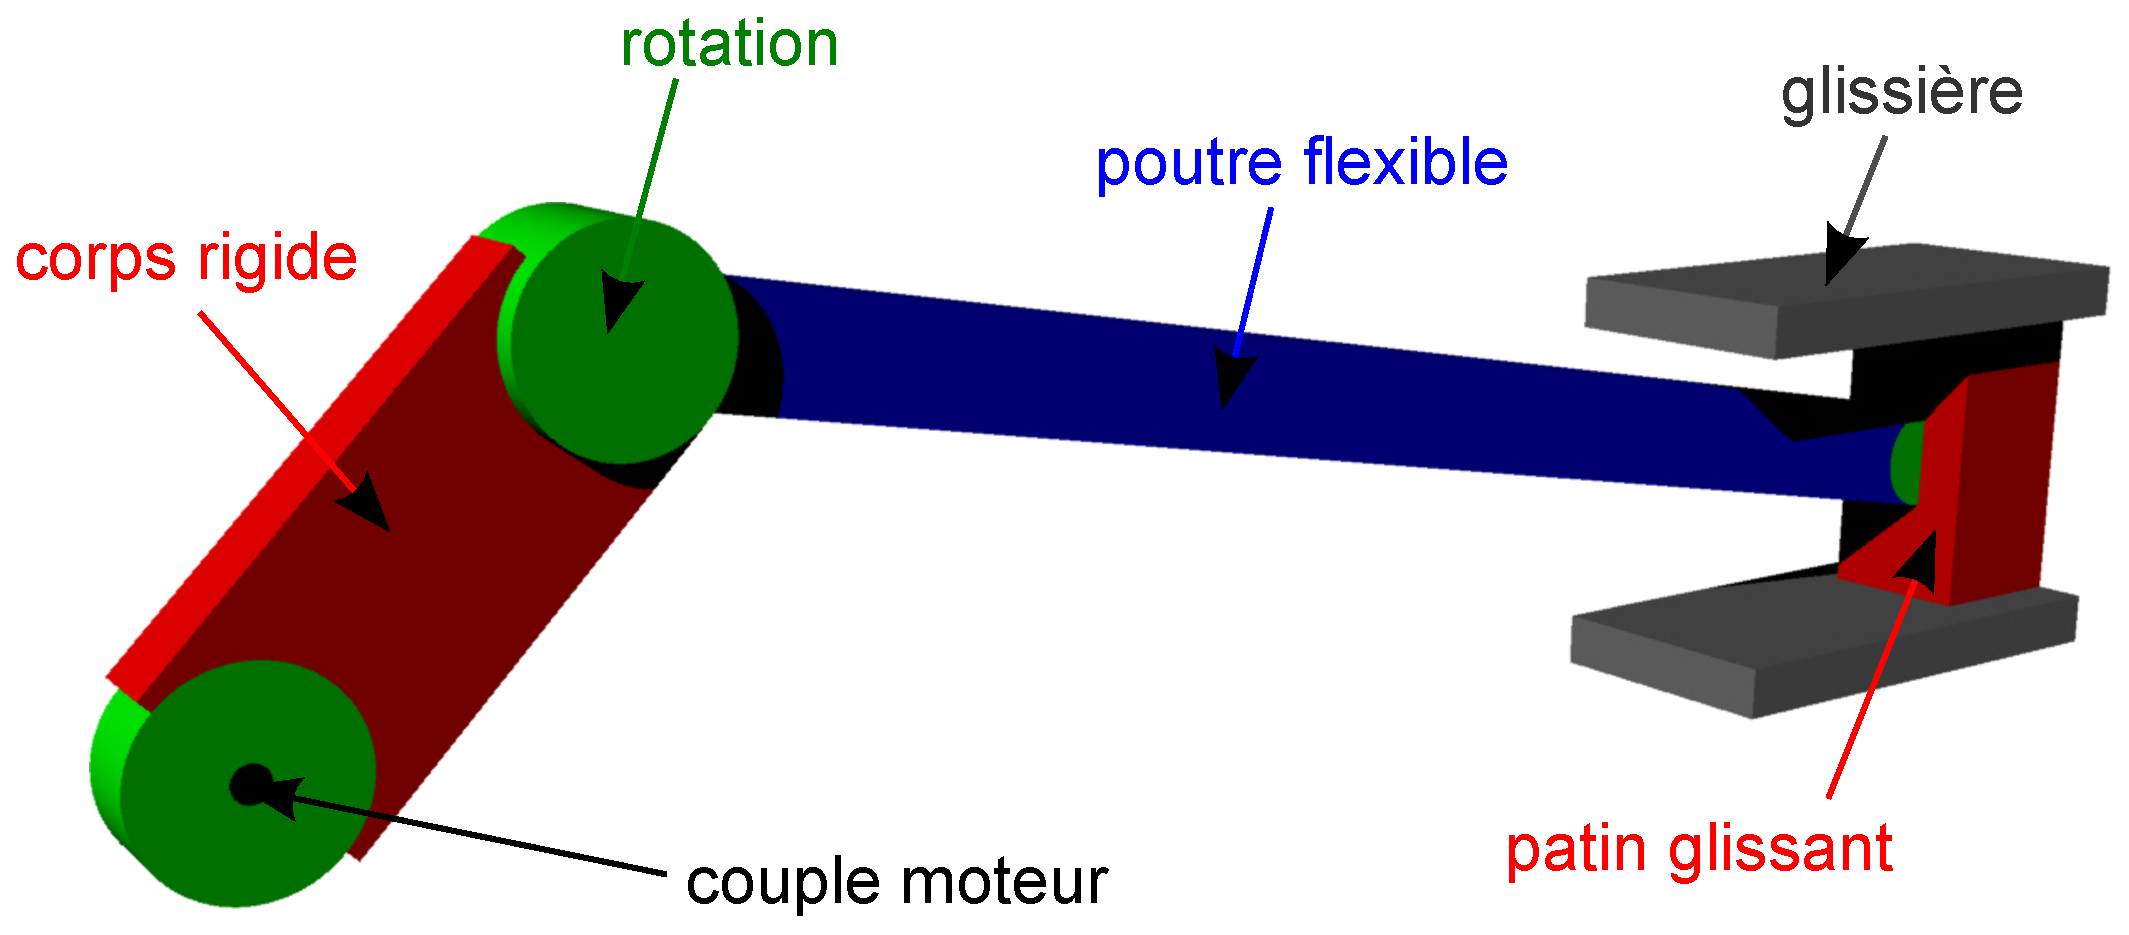
\includegraphics[height=45mm]{MBS}
\caption{Exemple de système multi-corps}
\end{figure}
\medskipvm
La dynamique d'un système multicorps est décrite par les équations du mouvement. On obtient alors un système de la forme:
\begin{equation}%
\left\{%
\begin{aligned}%
&M\ddot{u}-Q_{\dot{u}}+C_q\lambda = F\\
&C(u,\dot{u})=0
\end{aligned}\right.%
\end{equation}%
où~$M$ est la matrice de masse, $C$, la matrice des conditions de contraintes, $C_u$ la matrice jacobienne (dérivée de~$C$ par rapport à~$u$) permettant d'appliquer les forces~$\lambda$ correspondant à des multiplicateurs de Lagrange et~$Q_{\dot{u}}$, le vecteur de vitesse quadratique utilisé pour introduire les termes de Coriolis et les termes centrifuges.

\medskip
Nous n'entrons pas plus en avant, car le système à résoudre doit sembler suffisamment simple pour le lecteur à ce niveau du document et parce que cette méthode est d'application très particulière.
